% Useful: http://docs.latexlab.org

\documentclass[11pt]{article}
% used by \maketitle :
\title{DarkChat: a light weight, [almost] server-free, push-based robust p2p network with a chat payload}
\author{Nathan Griffith and Ahmet Aktay}
\date{May 12, 2010}
% used by \begin{code}:
\usepackage{fancyvrb}

\usepackage[utf8]{inputenc}
\usepackage[usenames,dvipsnames]{xcolor}
\usepackage{fullpage}
\usepackage[upright]{fourier}
\usepackage{tkz-graph}
\usetikzlibrary{arrows}


\DefineVerbatimEnvironment{code}{Verbatim}{fontsize=\small}
\DefineVerbatimEnvironment{example}{Verbatim}{fontsize=\small}
\newcommand{\ignore}[1]{}

\begin{document}
\maketitle % automatic title!

\section{Abstract}

The purpose of this project is to create a protocol for clients on a network to function with very little dependence on a server. In the case of \emph{DarkChat}, the clients function as 'chat' clients. The clients are able to communicate with each other information such as `online'/`offline' state and lists of contacts, with little-to-no interaction with the server.

While \emph{DarkChat} relies on a multi-threaded approach, and also makes no use of authentication, implementation decisions such as this have been made independently of the underlying protocol. As such, the protocal could be implemented in any number of ways, and this is meant as merely one example.

\section{Clients and Servers}

The `Client' class has been built as a wrapper for the messaging and interface classes, putting them all together into one usable chat client. Note that the term `client' is slightly misleading, as with the inclusion of a simple flag, a client can function as a server with very few implementation changes. It is possible that this could be reduced even further, such that servers could simply act as `super-clients' which store information about the entire netowrk, instead of about only their nearby edges and nodes.
In either case, the only purpose of the sever is to act as a secondary or backup repository for storing information about the network. Once the network is fully operational, the server is not needed, as long as enough clients remain online that one cluster of edges does not become separated from any other.

\subsection{Usage: Parameters}

When executing the client, a number of parameters can be passed. WIth the exception of `username' (`-u'), all parameters will revert to default values if none is specified:

\begin{code}
-p [port number, for accepting incoming communication]
-t [the default number of listening threads]
-u [the username of the client]
-sip [ip address of known server]
-sp [port number of known server]
-s (server flag, specifying that this instance of DarkChat is a server)
\end{code}

Note that there is currently no reliable centralized server, so in the actual case of starting a network running from scratch, it would be best to ensure that a server is running, and specify the server ip and port for each client. Once the clients are online and have contacted each other, one need only use a macro to contact a currently online client.

\subsection{Usage: Macros}

Once the client has been started, a number of macros have been made available to give the user control:

\begin{code}
  \help
   -Display this dialog
  \chat <username>
   -Switch to conversation with <username>
  \users
   -See a list of KNOWN users (online or off)
  \online
   -See a list of known, ONLINE users
  \offline
   -See a list of known, OFFLINE users
  \add <username>
   -Attempt to add username to list of known users
  \ping <ip> <port>
  -Attempt to ping the ip at the given port
  -If no port is specified, the current instance's incoming will be used
  \quit or \exit
   -Leave the program gracefully
\end{code}

Note that these are made available before the client has necessarly made successful contact with a server, allowing one to use the `\textbackslash ping' macro to manually connect to another client or server.

Once a connection has been made, information about offline and online users should propogate across the network and to the client, at which point the macros `\textbackslash online', `\textbackslash offline', and `\textbackslash users' will provide useful information.

To communcate with an online user, one need only use the `\textbackslash chat' macro (followed by the user's name) to start a new chat session with that user. From that point on, any line of text that is entered and doesn't start with a macro `\textbackslash' will be sent to \emph{all online sessons} associated with the reciever's username.\footnote{Currently there is no way to chat with \emph{only one} session if a user is logged into multiple.}

\section{The Algorithm}

While the details of the `Chat' client is useful in understanding some aspects of this algorithm, the true implementation has been abstracted from the end-user. Therefore, to understand the intent behind this project, a deeper explanation of the algorithm is required.

\subsection{The Network}

Instead of picturing the network in terms of `users' and `buddies' and `servers,' as one might with some types of chat implementations, one can also see it very simply as an undirected graph composed of nodes and edges. Each node represents a `client,' and each edge represents a direct, two-way association between two clients.\footnote{In the context of `chat,' adjacent nodes might represent ``buddies,'' but it's important to think of them abstractly.}

\begin{figure}
  \caption{An example network configuration}
  \begin{center}
  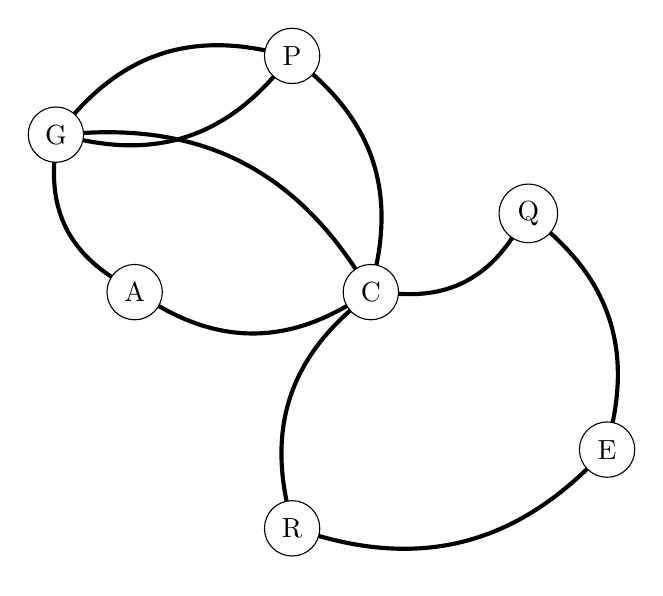
\begin{tikzpicture}
    \tikzstyle{VertexStyle}=[shape = circle, fill = white, minimum size = 20pt, text = black, draw]
    \SetUpEdge[lw         = 1.5pt,
                       color      = black,
                     labelcolor = white,
                      labeltext  = red,
                      labelstyle = {sloped,draw,text=blue}]
   \tikzstyle{EdgeStyle}=[bend left]
   \Vertex[x=0, y=4]{G}
   \Vertex[x=1, y=2]{A} 
   \Vertex[x=3, y=5]{P}
   \Vertex[x=4, y=2]{C}
   \Vertex[x=6, y=3]{Q}
   \Vertex[x=7, y=0]{E}
   \Vertex[x=3, y=-1]{R}
   \Edges(A,G,P,C)
   \Edges(Q,E,R,C,A)
   \Edges(P,G,C)  
   \Edges(Q,C)
  \end{tikzpicture}
  \end{center}
\label{graph}
\end{figure}

As shown in {\bf Figure \ref{graph}}, a network graph might look like one or more clusterings of nodes\footnote{This could be particularly true in the case of a `chat' client.}. In the \emph{DarkChat} implementation, each node is required to keep track of all nodes that are within two edge traversals.

When, for instance, a node is to add or update information about itself, it sends a notification to all nodes in its list of relevant nodes. This means that if, for instance, \emph{Node R} and \emph{Node E} have lost their connection to each other\footnote{This might happen if they have both changed IP addresses since their last communication}, they could rely on either \emph{Node C} or \emph{Node Q} to provide one of the required locations\footnote{Note that, of two nodes, only one need know the other's location in order for a connection to be established. In the case of \emph{E} and \emph{R}, as soon as \emph{Node E} sends a message to \emph{Node R}, the location of \emph{Node E} has been revealed.}.

Notice that \emph{Node C} is directly paired with all but \emph{Node E}, and even then \emph{E} and \emph{C} are within two edge traversals. This is a good example of a node with \emph{server-like} capabilities for this netork graph. However, since \emph{C} is in fact a client, this is a good example of the ways in which a server-free graph can still maintain robust and redundant connections for sending and recieiving updates.

THe final aspect of this graph worth noting is the fact that no server is shown. Presumably, all nodes would also be connected to some centralized server. However, under many normal conditions, this server would not be required. Only in cases where nodes are completely stranded would they \emph{need} to poll the server in order to maintain an accurate representation of their surrounding nodes. One such case might be if \emph{Node R} and \emph{Node E} are attempting to communicate with each other, and \emph{Node C} and \emph{Node Q} are both offline. As such, the more interconnected the clusters of nodes, the `healthier' the network.\footnote{This does not necessarily imply that the entire network is very interconnected, though this could also be the case. Instead, the `interconnectedness' implies only that many connections are shared within each cluster of nodes, of which there could be many.}

\subsection{The Status}

prune sessions -- compromising between age and online status

\subsection{The Protocol}

Clients make use of a limited number of message types to recieve the information they need.



\section{Use Cases}

NOT for high bandwidth cases -- if optimizing bandwidth is not as useful as increasing redundancy and synchronicity

Failsafes and backups -- gmail collapse -- the backups themselves are more of the 'same' -- failure mode is untested, anything causing original to go down causes backup.
In this case, the failure mode is being tested every day.

coordiation in case of an emergency

\section{Possible Optimizations}
scaling for bandwidth
   
message identifiers
   
combined requests

   
\begin{thebibliography}{1}

  \bibitem{prs}
    Atul Adya, John Dunagany, Alec Wolman,
    \emph{PRS: A Reusable Abstraction for Scaling Out Middle Tiers in the Datacenter}.
    Microsoft Research; Microsoft Corporation,
    2008.
\end{thebibliography}
\end{document}             % End of document.

